\documentclass{beamer}
%
% Choose how your presentation looks.
%
% For more themes, color themes and font themes, see:
% http://deic.uab.es/~iblanes/beamer_gallery/index_by_theme.html
%
\mode<presentation>
{
  \usetheme{Boadilla}      % or try Darmstadt, Madrid, Warsaw, ...
  \usecolortheme{default} % or try albatross, beaver, crane, ...
  \usefonttheme{default}  % or try serif, structurebold, ...
  \setbeamertemplate{navigation symbols}
} 

\usepackage[english]{babel}
\usepackage[utf8x]{inputenc}
\usepackage{pdfpages}
\usepackage{float}
\usepackage{ragged2e}
\usepackage{hyperref}

\newenvironment<>{varblock}[2][.9\textwidth]{%
  \setlength{\textwidth}{#1}
  \begin{actionenv}#3%
    \def\insertblocktitle{#2}%
    \par%
    \usebeamertemplate{block begin}}
  {\par%
    \usebeamertemplate{block end}%
  \end{actionenv}}

\title[Neuroanatomy workshop 3]{The Sensory-motor System}
\author{JJ Torre}
\institute{Parietal Team - INRIA Saclay}
\date{2018}

\begin{document}

\begin{frame}
  \titlepage
\end{frame}

% Uncomment these lines for an automatically generated outline.
%\begin{frame}{Outline}
%  \tableofcontents
%\end{frame}

\section{Introduction}

\begin{frame}{Introduction}
 \begin{columns}[T]
  \begin{column}{.4\textwidth}
    \begin{itemize}
    \justifying
      \item The sensory-motor system constitutes our main means of receiving input (sensory
      stimuli) and producing output (movement) in relation to the environment
      \item It follows a hierarchical organization common to both motor and sensory systems
    \end{itemize}

    \vspace{-.3cm}
    \begin{varblock}[5cm]{\scriptsize Peripheral Nervous System (PNS)}
    \justifying
     \scriptsize Although we are going to focus on the central nervous system, a lot is going on before reaching the brain! Motor reflexes happen at this level
    \end{varblock}
  \end{column}
  \begin{column}{.6\textwidth}
   \begin{figure}[H]
   \vspace*{-1.25cm}
    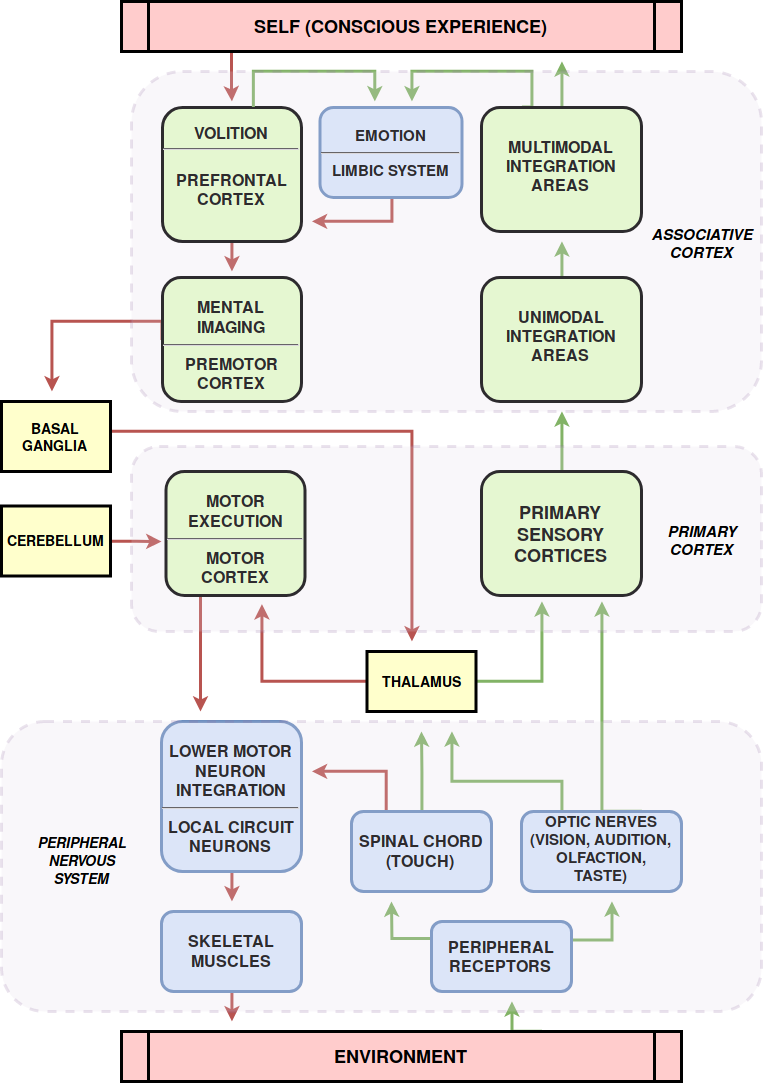
\includegraphics[width=.85\textwidth]{figures/brain_and_env.png}
   \end{figure}
  \end{column}
 \end{columns}
\end{frame}

\begin{frame}{Primary Areas}
 \begin{columns}[T]
  \begin{column}{.4\textwidth}
    \begin{itemize}
      \item \small Primary areas receive input directly from the thalamus
      \item \small Sensory areas receive high-dimensional data for each modality (vision, audition, etc.)
      \item \small The motor cortex conveys the already planned movement and sends it to the muscles
      \item \small Primary cortices have the better and most differentiated 6-layer laminar structure
    \end{itemize}
  \end{column}
  \begin{column}{.6\textwidth}
   \begin{figure}[H]
    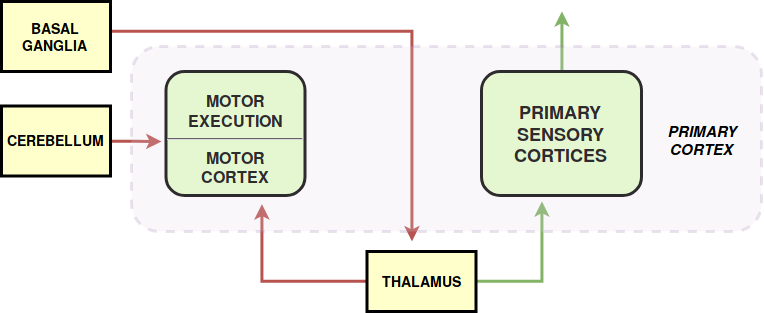
\includegraphics[width=1\textwidth, height=3.5cm]{figures/primary_structures.png}
   \end{figure}
   \vskip
   \begin{varblock}[7cm]{\scriptsize Olfaction is a special boy}
   \justifying
    \scriptsize Olfaction is the only sense that does not do thalamic relay in its
    path to the cortex. Signals from the nose go directly to the piriform cortex via the
    olfactory tract.
   \end{varblock}
  \end{column}
 \end{columns}
\end{frame}

\begin{frame}{Associative areas}

 \begin{columns}[T]
  \begin{column}{.4\textwidth}
    \begin{itemize}
      \item \small Can receive input from a diverse range of cortical areas
      \item \small As we move from primary to associative, it becomes ingreasingly difficult to pin down specific processes to brain regions
      \item \small There are two different sub-categories of associative areas: secondary (premotor cortex/unimodal integration areas) and tertiary (prefrontal cortex/multimodal integration)
    \end{itemize}
  \end{column}
  \begin{column}{.6\textwidth}
   \begin{figure}[H]
    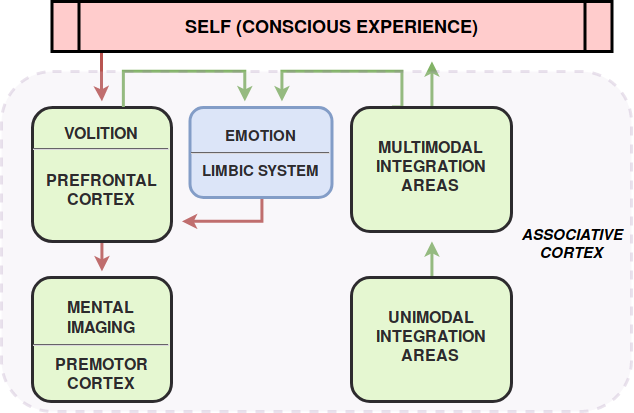
\includegraphics[width=.8\textwidth, height=3.5cm]{figures/associative_cortex.png}
    \end{figure}
   \vskip
   \begin{varblock}[7cm]{\scriptsize Neuroscientists do not agree on anyting - Part I}
   \justifying
    \scriptsize Although sometimes the term "associative" is used to designate all the cortex that is not a primary area, here we are referring only to sensory and motor association cortices.
   \end{varblock}
  \end{column}
 \end{columns}
\end{frame}

\begin{frame}{Secondary areas}

    \begin{itemize}
    \justifying
      \item They receive input mostly from their respective primary (sensory) or tertiary (motor) areas
      \item Secondary sensory areas show asymmetry patterns within each modality (more on that later)
      \item Secondary or premotor areas are mostly involved in the integration of all elements needed to perform movements
    \end{itemize}
    
\end{frame}

\begin{frame}{Tertiary areas}

    \begin{itemize}
    \justifying
      \item They constitute the link between higher cognition and their corresponding sensorimotor systems
      \item Information integrated from cognition that results in movement is feeded to secondary motor areas from tertiary motor areas, whereas tertiary sensory areas feed sensory representations to a variety of cortical areas
      \item The thalamus plays a crucial role in the widespread distribution both to and from these areas
      \item Processing in these areas does not involve perception or motor activities. Rather, they take charge of issue movements or integrate sensory representations across different sensory modalities
    \end{itemize}

\end{frame}

\section{The Motor System}

\begin{frame}{The Motor System: Function}

 \begin{columns}[T]
  \begin{column}{.5\textwidth}
  \vspace{.4cm}
    \begin{itemize}
    \justifying
      \item Unsurprisingly, it is in charge of controlling voluntary movements
      \item It is also in charge of controlling posture with the help of the vestibular system
      \item The primary motor cortex can be found anterior to the central sulcus. The premotor areas can be found anterior to the primary motor cortex. Both of them extend to the medial surface of the brain until the paracingulate sulcus
    \end{itemize}

  \end{column}
  \begin{column}{.6\textwidth}
   \begin{figure}[H]
   \vspace{-1.5cm}
    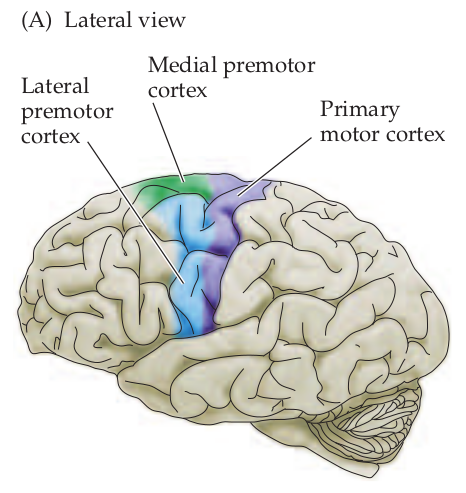
\includegraphics[width=.6\textwidth]{figures/motor_lateral.png}
   \end{figure}
   \vspace{-1cm}
   \begin{figure}[H]
    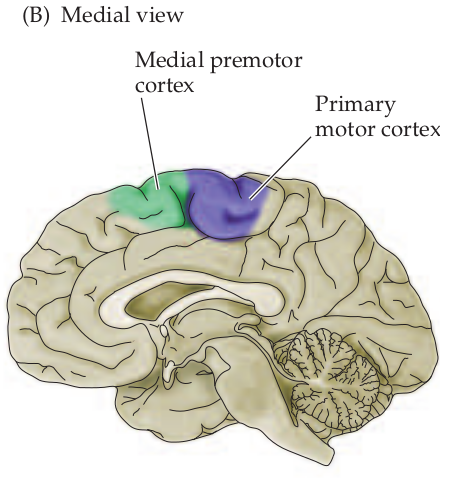
\includegraphics[width=.6\textwidth]{figures/motor_medial.png}
   \end{figure}
  \end{column}
 \end{columns}
    
\end{frame}

\begin{frame}{Primary Motor Cortex}

 \begin{columns}[T]
  \begin{column}{.5\textwidth}
   \vspace{.5cm}
    \begin{itemize}
    \justifying
      \item Follows a topographic organization of the body
      \item Each area contains populations of neurons specialized in movements rather than in innervating certain muscles
      \item The thalamus exerts a tonic inhibition on the motor system, and lifts this inhibition for areas where a movement is intended to be issued
    \end{itemize}

  \end{column}
  \begin{column}{.6\textwidth}
  \vspace{-.5cm}
   \begin{figure}[H]
    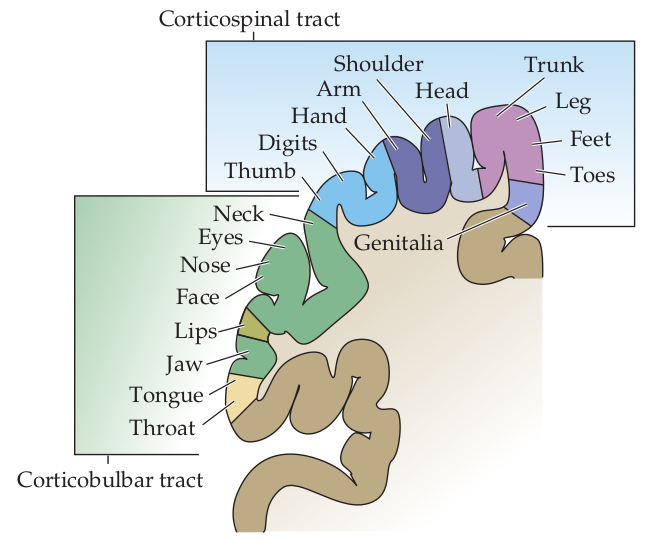
\includegraphics[width=.9\textwidth]{figures/primary_motor.png}
   \end{figure}
   
   
   \begin{varblock}[6.5cm]{\scriptsize Everything is crossed in the brain}
    \scriptsize As a rule of thumb, the brain processes information of the contralateral side of the body. Left hemisphere controls right side, and vice-versa
   \end{varblock}
  \end{column}
 \end{columns}
    
\end{frame}

\begin{frame}{Premotor Cortex}

    \begin{itemize}
    \justifying
      \item The premotor cortex uses information from other cortical areas to select movement appropiate to the context of the action
      \item The connections of this area are different when executing known moves in opposition to new moves
      \item In the case of new movements, they can be executed from observation or from memory, with different connections involved
   \end{itemize}
      
    \begin{varblock}[12cm]{Imagine your movements}
    \justifying
    If you "imagine" to move your arm, you can feel what it is like to activate this area of the brain witout ever reaching the actual motor cortex or muscles. This phenomenon applied to sports, music, and other areas is often called "mental play", and has shown strikingly effects in both profeesional musicians and sports players when used in addition to regular practice
    \end{varblock}

\end{frame}

\begin{frame}{Premotor Cortex}

    \begin{itemize}
    \justifying
      \item The medial premotor cortex has been shown to fire in presence of the cue in learning experiments. It is linked to movement intention elicited by external elements
      \item On the contrary, medial premotor cortex has been shown to reflect the intention of movements
      elicited by internal elements
      \item Some of the relevant cortical areas connected to the premotor cortex include: Angular and Supramarginal gyrus (mental "blueprints" of movements), Cerebellum (coordination of movements), Basal Ganglia (motor gating, automatization)
   \end{itemize}
   
   \begin{varblock}[12cm]{\small Trivia: Does cognition "move"?}
   \justifying
   \small Although the Cerebellum is usually seen as the "motor coordination system", there are specific parts of the cerebellum that are specialized in cognitive and emotional processing. Cerebellar lesions have been shown to affect high-order cognitive functions. This phenomenon receives the name "dysmetria of thought"
   \end{varblock}

\end{frame}

\begin{frame}{Types of movements}
    
   \begin{itemize}
       \item There are three types of movements, broadly speaking:
        \begin{itemize}
        \justifying
            \item Stereotypical: Automatic and usually innate. No cortical activity involved. \textbf{Examples}: knee-jerk reflex, vestibulo-ocular reflex 
            \item Rhythmic and coordinated: Require visuo-motor coordination, as well as muscular tone, equilibrium, etc. Their initiation is voluntary but the process is automatic. \textbf{Example}: walking
            \item Learned: Require constant cortical adjustment and attention. Highly complex and often manipulative
        \end{itemize}
        \bigskip
       \item There are also two types of gestures or simple movements:
        \begin{itemize}
        \justifying
            \item Transitive: They require tools. Usually goal-oriented. \textbf{Examples}: Hammering a nail, smoking a cigarette
            \item Intransitive: Do not require tools. Usually communication-oriented. \textbf{Examples}: Waving hello/goodbye, showing approval with a thumbs up
        \end{itemize}
   \end{itemize}
\end{frame}

\begin{frame}{The Motor System: Dysfunction}

 \begin{columns}[T]
  \begin{column}{.55\textwidth}
    \begin{itemize}
    \justifying
      \item Damage to the primary motor cortex or any point of the pathways that connect it with the skeletal muscles result in impairment or loss of motor function
      \item Depending on the point of the lesion, the symptoms are different:
       \begin{itemize}
       \justifying
       \vspace{.3cm}
           \item \scriptsize If damage is done to the motor cortex or any area in the descending pathways, it produces what is known as \textbf{Upper Motor Neuron Syndrome}. It can be ipsi or contralateral
           \item \scriptsize On the contrary, damage to any point of the pathway from the synapsis at the brain stem (face) or spinal cord (body) will give rise to the \textbf{Lower Motor Neuron Syndrome}. Its effect are always ipsilateral
       \end{itemize}
       
    \end{itemize}
  \end{column}
  \begin{column}{.5\textwidth}
   \begin{figure}[H]
   \vspace{-1.5cm}
    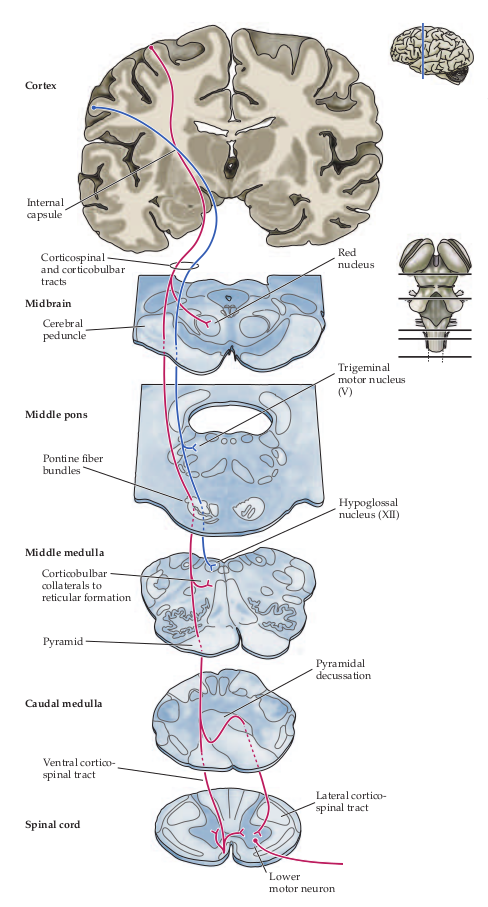
\includegraphics[width=.8\textwidth]{figures/motor_pathway.png}
    \end{figure}
  \end{column}
 \end{columns}
 
\end{frame}

\begin{frame}{Associative deficits: Apraxia}

 \begin{itemize}
 \justifying
     \item The term "apraxia" refers to a disorder where a patient is unable to perform daily life movements, with motor functions being preserved
     \item Some patients present difficulties performing movements when verbally instructed to do so, and others present difficulties to imitate movements
     \item They can have their origin in focal lesions of areas involved in motor planning, or lesions on the white matter tracts that connect them
     \item There are two major types of motor apraxia: Ideomotor apraxia and Ideational apraxia
 \end{itemize}
    
\end{frame}

\begin{frame}{Ideomotor apraxia}
 \begin{itemize}
 \justifying
     \item \small Difficulty to perform learned movements. Specially those that require tools, but not always
     \item \small Problems can be only with the tool, only without it, only when instructed to perform the movement or only when asked to imitate a movement
     \item \small The origin is usually a lesion on the parietal cortex in charge of the mental representations, in the premotor cortex or in the conexion between them
     \item \small Depending on the origin of the lesion, the patient can preserve the mental representation ("I know what I have to do, but I can't do it) or not ("I can't remember how to do it")
     \item \small \href{https://www.youtube.com/watch?v=EvOYeqM-6CE}{Video example}
 \end{itemize}
 
 \begin{varblock}[12cm]{\small Apraxia does not affect politeness}
 \justifying
 \small Althought it is fairly common that apraxic patients are unable to wave hello or goodbye when instructed to, it is a curious occurrence to see that the spontaneously do it when arriving or leaving. The key is that waving in these kinds of scenarios is \textit{automatic}, so some argue that other pathways are implied in that particular action
 
 \end{varblock}
    
\end{frame}

\begin{frame}{Ideational apraxia}

 \begin{itemize}
 \justifying
     \item Also known as conceptual apraxia, has its roots in more sophisticated planning and goal-oriented behaviors
     \item The patient presents impairment or inability to perform complex sequence of movements, like frying an egg, lighting a candle with a match, or putting a letter in an envelope
     \item This type of apraxia does not appear after brain traumatism or stroke, it appears in neurodegenerative diseases
     \item Here, the mental concepts linked to the steps of the sequence are damaged or lost, the range of particular symptoms is wide. The patient is unable to explain the process or its goals, as higher representations of the requested behavior are compromised
 \end{itemize}
    
\end{frame}

\begin{frame}{Other types of apraxia}

 \begin{itemize}
 \justifying
     \item \textbf{Limb apraxia}: Similar to ideomotor apraxia, but only with the arm contralateral to the lesion, and always preserving the mental representation of the movements. All types of performance (instruction, imitation, etc.) are impaired, as the origin is a disconnection between primary and secondary motor cortices
     \item \textbf{Oral apraxia}: Movements involving the face, tongue, cheeks and mouth are compromised. Can affect speech production. Insular/opercular lesions
     \item \textbf{Dressing apraxia}: Difficulties to dress, usually placing clothing in wrong parts of the body. Some argue that is a type of ideational apraxia.
     \item \textbf{Visoconstructive apraxia}: Impairment or inability to perform visually guided actions. Right and Left lesions present different symptomatology.
 \end{itemize}
    
\end{frame}

\end{document}
